% ============================================================
%  FORMULATION, DEVELOPMENT AND PRELIMINARY EVALUATION OF A
%  TRANSPARENT GEL FACE WASH CONTAINING SALICYLIC ACID
%  AND NEEM EXTRACT
%  Author: Purva Chordia | Guide: Madhuri Gahlod
% ============================================================
\documentclass[10pt,a4paper,twocolumn]{article}

%% ---- Encoding & font ----------------------------------------
\usepackage[T1]{fontenc}
\usepackage[utf8]{inputenc}
\usepackage{lmodern}

%% ---- Page layout --------------------------------------------
\usepackage[top=2.5cm,bottom=2.5cm,left=3cm,right=2.5cm]{geometry}
\usepackage{setspace}
\onehalfspacing

%% ---- Graphics & colour --------------------------------------
\usepackage{graphicx}
\usepackage[dvipsnames,svgnames,x11names]{xcolor}

%% ---- Tables -------------------------------------------------
\usepackage{booktabs}
\usepackage{tabularx}
\usepackage{array}
\usepackage{longtable}
\usepackage{multirow}
\usepackage{float}

%% ---- Maths --------------------------------------------------
\usepackage{amsmath}

%% ---- Lists --------------------------------------------------
\usepackage{enumitem}

%% ---- TikZ & pgfplots ----------------------------------------
\usepackage{tikz}
\usetikzlibrary{
  shapes.geometric, arrows.meta, positioning,
  fit, calc, backgrounds,
  decorations.pathreplacing, shadows
}
\usepackage{pgfplots}
\pgfplotsset{compat=1.18}

%% ---- Captions -----------------------------------------------
\usepackage{caption}
\usepackage{subcaption}

%% ---- Bibliography -------------------------------------------
\usepackage[numbers,sort&compress]{natbib}
\setcitestyle{super,square}
\bibliographystyle{unsrtnat}

%% ---- Hyperref (load last) -----------------------------------
\usepackage{microtype}
\usepackage[colorlinks=true,
            linkcolor=MidnightBlue,
            citecolor=MidnightBlue,
            urlcolor=MidnightBlue,
            pdftitle={Formulation of Transparent Gel Face Wash},
            pdfauthor={Purva Chordia}]{hyperref}

%% ---- TikZ global node styles --------------------------------
\tikzset{
  block/.style={
    rectangle, rounded corners=4pt,
    draw=SteelBlue!70, fill=SteelBlue!10,
    text width=4cm, minimum height=0.9cm,
    align=center, font=\small},
  greenblock/.style={
    rectangle, rounded corners=4pt,
    draw=ForestGreen!70, fill=ForestGreen!10,
    text width=5.5cm, minimum height=0.9cm,
    align=center, font=\small},
  redblock/.style={
    rectangle, rounded corners=4pt,
    draw=Crimson!70, fill=Crimson!8,
    text width=4.3cm, minimum height=0.9cm,
    align=center, font=\small},
  wideblock/.style={
    rectangle, rounded corners=4pt,
    draw=gray!60, fill=gray!8,
    text width=6cm, minimum height=0.9cm,
    align=center, font=\small},
  donebox/.style={
    rectangle, rounded corners=4pt,
    draw=Teal!70, fill=Teal!10,
    text width=5.6cm, minimum height=0.9cm,
    align=center, font=\small},
  todobox/.style={
    rectangle, rounded corners=4pt,
    draw=DarkOrange!70, fill=DarkOrange!10,
    text width=5.6cm, minimum height=0.9cm,
    align=center, font=\small},
  myarrow/.style={-Stealth, thick, gray!70},
}

% ============================================================

\usepackage{titlesec}
\titleformat{\section}
  {\normalfont\large\bfseries\color{Brown}}{}{0em}{}
\titleformat{\subsection}
  {\normalfont\normalsize\bfseries\color{Brown}}{}{0em}{}
\begin{document}

\twocolumn[{%
  \singlespacing
  \begin{center}
    {\Large\bfseries FORMULATION AND PRELIMINARY EVALUATION OF A TRANSPARENT GEL FACE WASH CONTAINING SALICYLIC ACID AND NEEM EXTRACT\par}
    \vspace{0.5cm}
    {\large\bfseries Purva Chordia$^{1}$, Madhuri Gahlod$^{2}$\par}
    \vspace{0.3cm}
    {\normalsize $^1$ \textit{B.Tech Cosmetic Technology, 3rd year, MGM University, Chh. Sambhajinagar.}\\
    $^2$ \textit{Assistant Professor, Department of Cosmetic Technology, MGM University, Chh. Sambhajinagar.}\par}
    \vspace{0.2cm}
    {\normalsize $^1$Corresponding Author: purvachordia40@gmail.com\\\normalsize $^2$Corresponding Author: profmdpardeshi@rediffmail.com\\ DOI: \href{https://doi.org/10.21831/jbsac.v2i2}{10.21831/jbsac.v2i2}\par}
    \vspace{0.3cm}
    \rule{\textwidth}{0.8pt}
    \vspace{0.3cm}
  \end{center}
  
  \noindent\begin{minipage}[t]{0.32\textwidth}
  {\color{Brown}\textbf{Article Info}}\par\vspace{0.2cm}
  Received: Day Month Year\par
  Accepted: Day Month Year\par
  Available online: Day Month Year\par
  \vspace{1cm}
  {\color{Brown}\textbf{Keywords}}\par\vspace{0.2cm}
  Salicylic acid;
Neem extract; gel face wash; acne-prone skin; 
preliminary evaluation.
  \end{minipage}%
  \hfill
  \begin{minipage}[t]{0.64\textwidth}
  {\color{Brown}\textbf{Abstract}}\par\vspace{0.2cm}
  Acne-prone skin is commonly associated with increased sebum production,
follicular obstruction, abnormal keratinization and inflammation, and
cleansing is an important part of skin care for oily and acne-prone skin.
Salicylic acid is widely used in topical acne-care products because of
its desmolytic and comedolytic properties, and neem
(\textit{Azadirachta indica}) has been investigated for antimicrobial,
anti-inflammatory and antioxidant properties. To develop a transparent gel face wash containing salicylic acid and
freshly prepared aqueous neem extract, and to carry out a preliminary
laboratory evaluation of its physical and sensory characteristics, fresh neem leaves were washed, crushed, extracted with water by heating,
cooled and filtered. Three laboratory batches (F1, F2 and F3) were
prepared with sodium lauryl ether sulphate (SLES) at 8\%, 10\% and 12\%
w/w, respectively, with all other listed components kept at the same
nominal levels. The selected batch, F2, was assessed qualitatively for
appearance, clarity, odour, colour, visible particles, phase separation,
uniformity, homogeneity, spreadability and skin feel. pH and viscosity
were not instrumentally determined, and no assay, microbiological,
preservative-efficacy, stability or clinical testing was performed. F2 was a pale-green, clear, uniform gel with a lime-like odour, without
visible particles or visible phase separation, and with good qualitative
spreadability and a pleasant subjective skin feel. F1 and F3 showed
similar visual characteristics but varied slightly in spreadability, 
skin feel, and foam height, supporting F2 as a balanced intermediate. The study shows the laboratory feasibility of preparing a transparent
gel face-wash formulation containing salicylic acid and fresh neem
extract. The findings are preliminary formulation-development observations
and are not evidence of anti-acne efficacy, antimicrobial activity,
preservative effectiveness, stability or safety. The methyl paraben level
used (1.5\% w/w) exceeds the limit permitted in the European Union and
should be revisited. Analytical, microbiological, stability and clinical
studies are required.
  \end{minipage}\par
  \vspace{0.5cm}
  \noindent\rule{\textwidth}{0.8pt}
  \vspace{0.5cm}
}]

% ============================================================
\section{INTRODUCTION}
% ============================================================

Acne vulgaris is a common inflammatory disorder of the pilosebaceous
unit that presents with comedones, papules and pustules. Topical,
light-based and complementary interventions for acne have been examined
in systematic reviews \citep{yuan2024}, and evidence-based guidelines
address both topical and systemic management
\citep{zaenglein2016,reynolds2024}. Factors associated with acne include
increased sebum production, abnormal follicular keratinization,
inflammation and microbial involvement \citep{zaenglein2016}. The most
recent American Academy of Dermatology guideline makes a conditional
recommendation for topical salicylic acid and supports combining topical
agents that act through different mechanisms \citep{reynolds2024}.

Cleansing is an important part of skin care for acne-prone skin
\citep{decker2012,delrosso2013}. A face wash is intended to remove
surface impurities, excess sebum and sweat while giving an acceptable
sensory experience, and a gel can offer a light, non-greasy, easily
spread dosage form for oily skin. Because surfactant-based cleansers can
affect the skin barrier, mildness is an important design consideration
\citep{ananthapadmanabhan2004,subramanyan2004}.

\subsection{Skin type and skin-surface pH}

The formulation was conceived for oily and acne-prone skin, in which
increased sebum output may contribute to accumulation of sebum and
cellular debris within follicles and hence to comedone formation. A
cleanser for this skin type should cleanse effectively without leaving a
heavy or greasy after-feel. Skin-surface pH is also relevant to cleanser
design: the natural skin-surface pH is acidic and averages below~5
\citep{lambers2006}, and higher facial skin pH has been reported in
patients with acne than in controls \citep{prakash2017}.

\subsection{Salicylic acid}

Salicylic acid is a lipophilic beta-hydroxy acid used in acne-care
products. It promotes desquamation by reducing corneocyte adhesion and
has comedolytic activity, which makes it relevant to formulations for
comedonal and oily skin \citep{decker2012,arif2015}. Although
historically classed as a keratolytic, it is now regarded as a
desmolytic agent because it disrupts cell junctions rather than lysing
intercellular keratin filaments \citep{arif2015}. Salicylic acid is used
at low concentrations in cleansers and other over-the-counter acne
products \citep{decker2012,arif2015}. In this study it was selected as
the defined active component. Its presence in a formulation does not by
itself establish clinical efficacy of a finished rinse-off product.

\subsection{Neem extract}

Neem (\textit{Azadirachta indica}) has a long history of use in
traditional skin-care preparations and contains many bioactive
constituents \citep{singh2021,kumar2013,gupta2017}. It has been
investigated for antimicrobial, anti-inflammatory and antioxidant
activities \citep{singh2021,kumar2013,gupta2017,alzohairy2016}; reported
constituents include nimbin, nimbidin, nimbolide and other limonoids, and
quercetin and $\beta$-sitosterol from fresh leaves have been reported to
show antibacterial and antifungal activity \citep{alzohairy2016}. Herbal
dermatological products are, however, subject to variability in
ingredient concentration and to quality-control and regulatory challenges
\citep{brar2025}. In this study freshly prepared aqueous neem extract
was used as a botanical formulation component. The extract was not
standardized for any phytoconstituent.

\subsection{Rationale}

The two ingredients were combined on the premise that they might
contribute complementary functions in a rinse-off gel: salicylic acid
through desmolytic and comedolytic action, and neem through its reported
antimicrobial and anti-inflammatory potential
(Figure~\ref{fig:rationale}). This is a formulation rationale drawn from
the literature
\citep{decker2012,arif2015,singh2021,kumar2013,gupta2017,alzohairy2016,brar2025},
not a demonstrated synergy. The study was designed as a laboratory-scale
formulation-development exercise focused on preliminary physical and
sensory characteristics. A marketed neem-based face wash was selected as
a descriptive commercial reference \citep{himalaya2026}.

%% ------ Figure 1 : Rationale diagram ------------------------
\begin{figure*}[t]
\centering
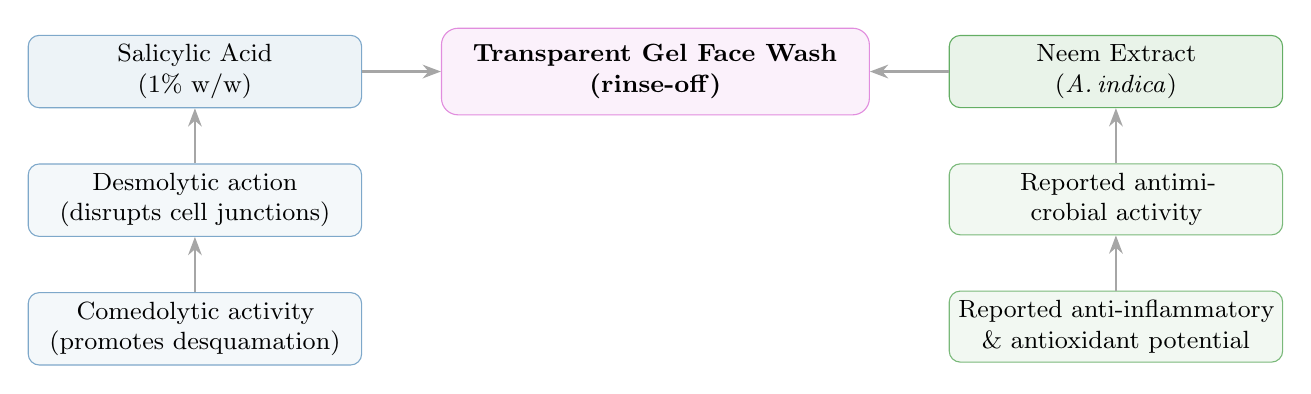
\begin{tikzpicture}[node distance=1.5cm and 2.5cm]
  %% Central product
  \node[rectangle, rounded corners=6pt,
        draw=Orchid!80, fill=Orchid!10,
        text width=5.2cm, minimum height=1.1cm,
        align=center, font=\small\bfseries] (product)
    {Transparent Gel Face Wash\\(rinse-off)};

  %% Salicylic acid (left)
  \node[block, left=1cm of product] (sa)
    {Salicylic Acid\\(1\% w/w)};
  \node[block, below=0.7cm of sa, fill=SteelBlue!6] (sa1)
    {Desmolytic action\\(disrupts cell junctions)};
  \node[block, below=0.7cm of sa1, fill=SteelBlue!6] (sa2)
    {Comedolytic activity\\(promotes desquamation)};

  %% Neem (right)
  \node[block, right=1cm of product,
        draw=ForestGreen!70, fill=ForestGreen!10] (neem)
    {Neem Extract\\(\textit{A.\,indica})};
  \node[block, below=0.7cm of neem,
        draw=ForestGreen!60, fill=ForestGreen!6] (n1)
    {Reported antimicrobial activity};
  \node[block, below=0.7cm of n1,
        draw=ForestGreen!60, fill=ForestGreen!6] (n2)
    {Reported anti-inflammatory \&\ antioxidant potential};



  %% Arrows
  \draw[myarrow] (sa)   -- (product);
  \draw[myarrow] (neem) -- (product);
  \draw[myarrow] (sa2)  -- (sa1);
  \draw[myarrow] (sa1)  -- (sa);
  \draw[myarrow] (n2)   -- (n1);
  \draw[myarrow] (n1)   -- (neem);
\end{tikzpicture}
\caption{Schematic of the proposed complementary rationale for salicylic
acid (comedolytic, desmolytic) and neem extract (reported antimicrobial,
anti-inflammatory and antioxidant potential) in a rinse-off gel face
wash, based on the literature
\citep{decker2012,arif2015,singh2021,kumar2013,gupta2017,alzohairy2016,brar2025}.
The combined action was not tested in this study.}
\label{fig:rationale}
\end{figure*}



% ============================================================
\subsection*{Materials}
The ingredients and their intended functions are summarized in Table~\ref{tab:ingredients}.
% ============================================================

\begin{table*}[!htbp]
\centering

\renewcommand{\arraystretch}{1.35}
\begin{tabularx}{\textwidth}{>{\bfseries}lX}
\toprule
Ingredient & Intended function in the formulation \\
\midrule
Salicylic acid & Active ingredient \\
Fresh neem leaves & Source of aqueous botanical extract \\
Sodium lauryl ether sulphate (SLES) & Primary cleansing surfactant \\
Sodium lauryl sulphate (SLS) & Co-surfactant / foaming surfactant \\
Carbopol 940 & Gelling agent \\
Lime water & Fragrance / formulation ingredient (identity and composition
             not documented; see Section~\ref{sec:discussion}) \\
Glycerol & Humectant \\
Methyl paraben & Preservative (the only paraben used; propyl paraben was
                 not used) \\
Triethanolamine (TEA) & Carbopol neutralizer; gel development \\
Distilled water & Vehicle (q.s.\ to final weight) \\
\bottomrule
\end{tabularx}
\caption{Ingredients and their intended functions}
\label{tab:ingredients}
\end{table*}

Methyl paraben has been used as an antimicrobial preservative in foods,
drugs and cosmetics for more than 50 years \citep{soni2002}. No water
bath, pH meter or viscometer was used in this work; equipment was used
according to availability. Ingredient grades, suppliers and batch numbers
were not recorded.

% ============================================================
\section{METHOD}
% ============================================================

\subsection{Preparation of neem extract}

Fresh neem leaves were selected and washed with water to remove visible
dirt and foreign matter. The leaves were crushed to increase the surface
area available for extraction, soaked in water and heated to boiling.
The mixture was cooled and filtered to remove plant material, and the
filtrate was used as the neem extract (Figure~\ref{fig:neemextract}).
Leaf mass, solvent volume, extraction temperature, extraction time and
extract yield were not recorded, and the extract was not standardized.

%% ------ Figure 2 : Neem extraction flowchart ---------------
\begin{figure*}[t]
\centering
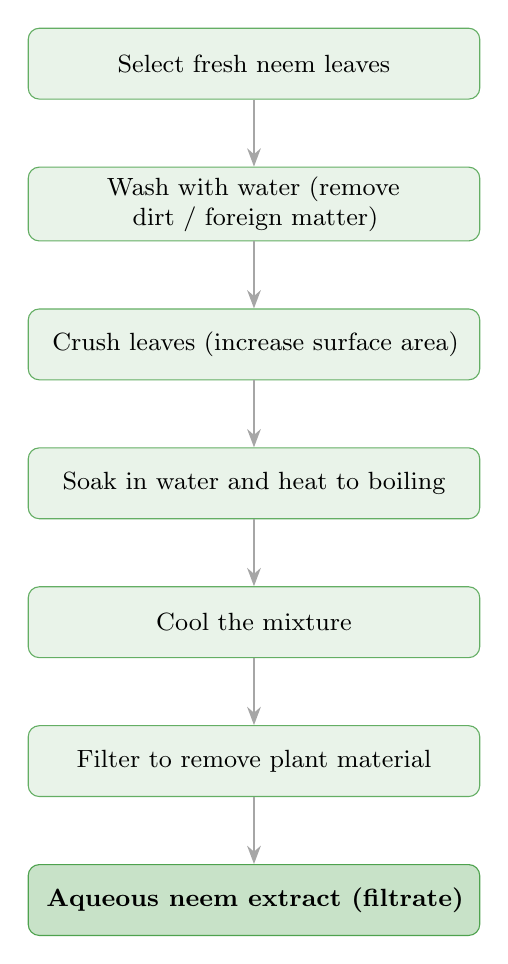
\begin{tikzpicture}[node distance=0.85cm]
  \node[greenblock] (s1) {Select fresh neem leaves};
  \node[greenblock, below=of s1] (s2)
    {Wash with water (remove dirt / foreign matter)};
  \node[greenblock, below=of s2] (s3)
    {Crush leaves (increase surface area)};
  \node[greenblock, below=of s3] (s4)
    {Soak in water and heat to boiling};
  \node[greenblock, below=of s4] (s5) {Cool the mixture};
  \node[greenblock, below=of s5] (s6)
    {Filter to remove plant material};
  \node[greenblock, below=of s6,
        fill=ForestGreen!25, draw=ForestGreen!80,
        font=\small\bfseries] (s7)
    {Aqueous neem extract (filtrate)};

  \foreach \a/\b in {s1/s2,s2/s3,s3/s4,s4/s5,s5/s6,s6/s7}
    \draw[myarrow] (\a)--(\b);
\end{tikzpicture}
\caption{Preparation of aqueous neem extract from fresh neem leaves. Leaf
mass, solvent volume, extraction temperature, time and yield were not
recorded.}
\label{fig:neemextract}
\end{figure*}

\subsection{Formulation design}

Three batches were prepared in which SLES was the only intentionally
varied component (8\%, 10\% and 12\% w/w in F1, F2 and F3,
respectively). SLS, salicylic acid, lime water, glycerol, Carbopol~940,
methyl paraben and neem extract were held at the same nominal levels
(Table~\ref{tab:composition}, Figure~\ref{fig:composition}). The nominal
water contents in the original batch sheet (82.8\%, 80.8\% and 78.8\%)
summed to exactly 100\% without any allowance for triethanolamine; water
is therefore reported as q.s.\ to 100\%, with the nominal values shown
for reference.

\begin{table*}[!htbp]
\centering

\renewcommand{\arraystretch}{1.3}
\begin{tabularx}{\textwidth}{lccclX}
\toprule
\textbf{Ingredient} & \textbf{F1} & \textbf{F2 (selected)} &
\textbf{F3} & \textbf{Function} \\
\midrule
SLES             & 8    & 10   & 12   & Cleansing surfactant \\
SLS              & 1    & 1    & 1    & Co-surfactant \\
Salicylic acid   & 1    & 1    & 1    & Active ingredient \\
Lime water       & 2    & 2    & 2    & Fragrance / ingredient \\
Glycerol         & 2    & 2    & 2    & Humectant \\
Carbopol 940     & 0.7  & 0.7  & 0.7  & Gelling agent \\
Methyl paraben   & 1.5  & 1.5  & 1.5  & Preservative \\
Neem extract     & 1    & 1    & 1    & Botanical ingredient \\
Triethanolamine  & q.s. & q.s. & q.s. & Neutralizer (see text) \\
Distilled water  & \multicolumn{1}{l}{q.s.\ to 100}
                 & \multicolumn{1}{l}{q.s.\ to 100}
                 & \multicolumn{1}{l}{q.s.\ to 100}
                 & Vehicle \\
                 & \multicolumn{1}{l}{(nominal 82.8)}
                 & \multicolumn{1}{l}{(nominal 80.8)}
                 & \multicolumn{1}{l}{(nominal 78.8)} & \\
\bottomrule
\end{tabularx}
\caption{Nominal composition of batches F1--F3 (\% w/w)}
\label{tab:composition}
\end{table*}

Triethanolamine was added dropwise (about 1--2 drops) until the gel
formed. Batch size and dropper calibration were not recorded, so the
quantity cannot be stated as a percentage. For illustration only,
assuming about 20~drops/mL and a density of about 1.12~g/mL, 1--2 drops
correspond to roughly 0.056--0.112~g, which would be about 0.06--0.11\%
w/w in a 100~g batch. The measured mass should be recorded in future
batches. The methyl paraben level (1.5\% w/w) exceeds the maximum of
0.4\% (as acid) permitted for a single paraben ester in cosmetic products
by Annex~V of Regulation~(EC) No~1223/2009 of the European Union; this
is discussed in Section~\ref{sec:discussion}.

%% ------ Figure 3 : Composition charts ----------------------
\begin{figure*}[t]
\centering
\begin{subfigure}[t]{0.55\textwidth}
\centering
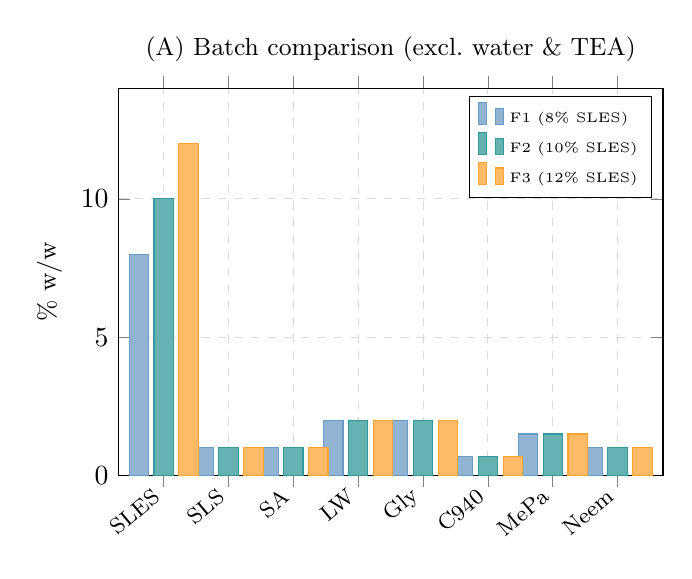
\begin{tikzpicture}
\begin{axis}[
  ybar, bar width=7pt,
  width=8.5cm, height=6.5cm,
  symbolic x coords={SLES,SLS,SA,LW,Gly,C940,MePa,Neem},
  xtick=data,
  xticklabel style={rotate=40, anchor=east, font=\footnotesize},
  ymin=0, ymax=14,
  ylabel={\% w/w}, ylabel style={font=\small},
  legend style={at={(0.98,0.98)}, anchor=north east,
                font=\tiny, cells={anchor=west}},
  title={\small (A) Batch comparison (excl.\ water \& TEA)},
  grid=major, grid style={dashed,gray!30},
]
\addplot+[fill=SteelBlue!60, draw=SteelBlue!80]
  coordinates{(SLES,8)(SLS,1)(SA,1)(LW,2)(Gly,2)
              (C940,0.7)(MePa,1.5)(Neem,1)};
\addplot+[fill=Teal!60, draw=Teal!80]
  coordinates{(SLES,10)(SLS,1)(SA,1)(LW,2)(Gly,2)
              (C940,0.7)(MePa,1.5)(Neem,1)};
\addplot+[fill=DarkOrange!60, draw=DarkOrange!80]
  coordinates{(SLES,12)(SLS,1)(SA,1)(LW,2)(Gly,2)
              (C940,0.7)(MePa,1.5)(Neem,1)};
\legend{F1 (8\% SLES), F2 (10\% SLES), F3 (12\% SLES)}
\end{axis}
\end{tikzpicture}
\end{subfigure}
\hfill
\begin{subfigure}[t]{0.42\textwidth}
\centering
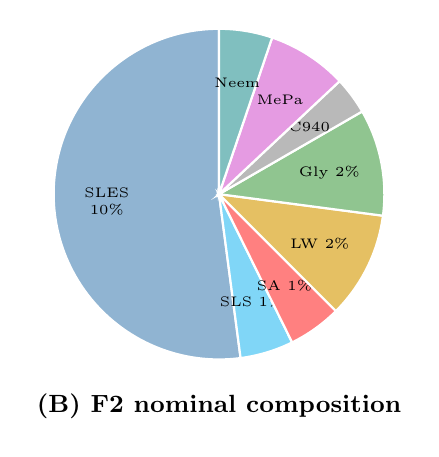
\begin{tikzpicture}
%% Pie chart for F2 (excluding water & TEA; total = 19.2)
%% Angles: SLES=10->187.5, SLS=1->18.75, SA=1->18.75,
%%         LW=2->37.5, Gly=2->37.5, C940=0.7->13.125,
%%         MePa=1.5->28.125, Neem=1->18.75
\def\R{2.1}
\def\pslice#1#2#3#4{%
  \pgfmathsetmacro{\midangle}{(#1+#2)/2}
  \fill[#4] (0,0) -- (#1:\R) arc(#1:#2:\R) -- cycle;
  \draw[white, line width=0.8pt] (0,0) -- (#1:\R) arc(#1:#2:\R) -- cycle;
  \node[font=\tiny, align=center] at (\midangle:0.68*\R) {#3};
}
\begin{scope}
  \pslice{90}{277.5}{SLES\\10\%}{SteelBlue!60}
  \pslice{277.5}{296.25}{SLS 1\%}{cyan!50}
  \pslice{296.25}{315}{SA 1\%}{red!50}
  \pslice{315}{352.5}{LW 2\%}{Goldenrod!70}
  \pslice{352.5}{390}{Gly 2\%}{ForestGreen!50}
  \pslice{390}{403.125}{C940}{gray!55}
  \pslice{403.125}{431.25}{MePa}{Orchid!70}
  \pslice{431.25}{450}{Neem}{Teal!50}
\end{scope}
\node[font=\small\bfseries] at (0,-2.7)
  {(B) F2 nominal composition};
\end{tikzpicture}
\end{subfigure}
\caption{(A) Nominal ingredient levels (\% w/w, excluding water and
triethanolamine) of batches F1, F2 and F3; only SLES varies between
batches. (B) Nominal composition of the selected batch F2.
Triethanolamine (q.s.; about 1--2 drops) is not shown.
SA\,=\,salicylic acid; LW\,=\,lime water; Gly\,=\,glycerol;
C940\,=\,Carbopol~940; MePa\,=\,methyl paraben.}
\label{fig:composition}
\end{figure*}

\subsection{General formulation procedure}

Carbopol~940 was dispersed gradually in distilled water and allowed to
hydrate. SLES and SLS were incorporated with gentle stirring to minimize
foam formation. Glycerol, lime water and the freshly prepared neem
extract were then added, followed by gradual addition of salicylic acid
with continuous mixing. Methyl paraben was added as the intended
preservative. Triethanolamine was added in small quantity to neutralize
the Carbopol and develop the gel structure, and the preparation was made
up to final weight with distilled water and mixed until visually uniform
(Figure~\ref{fig:procedure}). Mixing speed and duration, hydration time,
temperature, batch size and final batch weight were not recorded.

Excipients were chosen for defined roles. Carbopol~940, once neutralized,
forms a microgel that has been characterized as an effective
dermatological gel base, and its rheology depends on the neutralization
pH \citep{islam2004}. Glycerol is a humectant and endogenous skin
component that has been reported to improve stratum corneum hydration and
barrier function \citep{fluhr2008}. SLES and SLS provide cleansing and
foaming, and, because surfactant-based cleansers can affect the skin
barrier \citep{ananthapadmanabhan2004,subramanyan2004}, the SLES level
was chosen as the variable of interest.

%% ------ Figure 4 : Formulation procedure -------------------
\begin{figure*}[t]
\centering
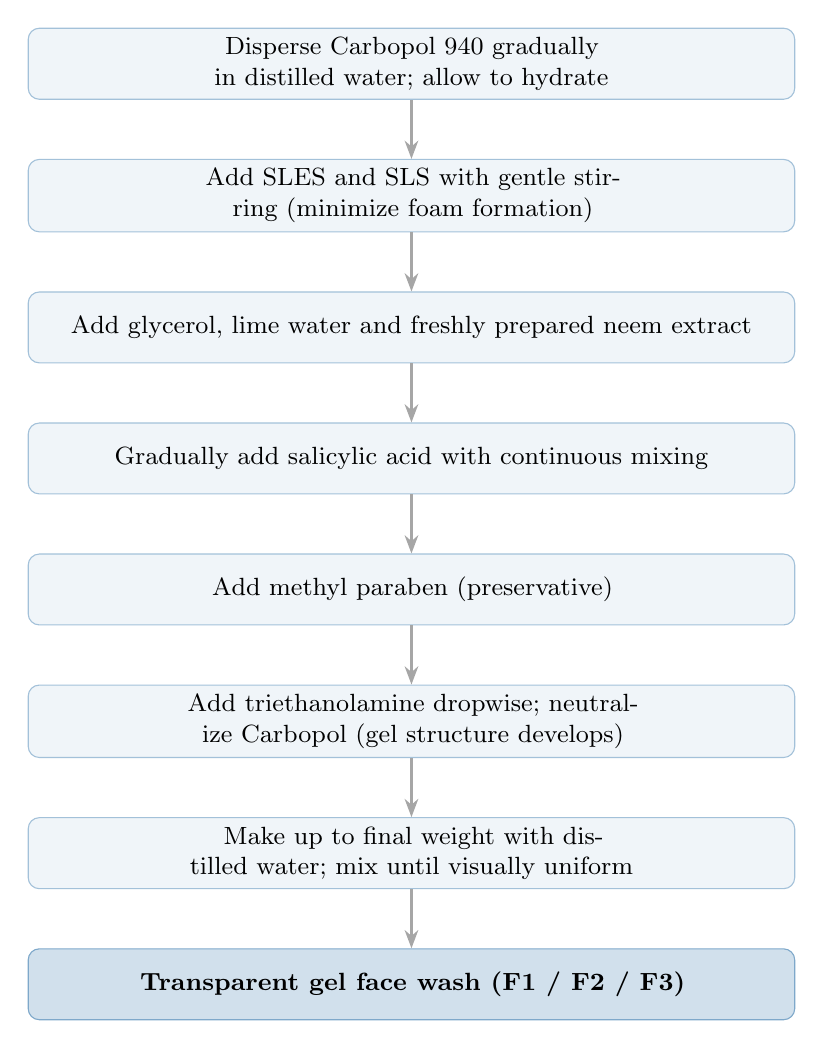
\begin{tikzpicture}[node distance=0.75cm]
  \node[wideblock, text width=9.5cm, fill=SteelBlue!8,
        draw=SteelBlue!50] (p1)
    {Disperse Carbopol~940 gradually in distilled water; allow to hydrate};
  \node[wideblock, text width=9.5cm, fill=SteelBlue!8,
        draw=SteelBlue!50, below=of p1] (p2)
    {Add SLES and SLS with gentle stirring (minimize foam formation)};
  \node[wideblock, text width=9.5cm, fill=SteelBlue!8,
        draw=SteelBlue!50, below=of p2] (p3)
    {Add glycerol, lime water and freshly prepared neem extract};
  \node[wideblock, text width=9.5cm, fill=SteelBlue!8,
        draw=SteelBlue!50, below=of p3] (p4)
    {Gradually add salicylic acid with continuous mixing};
  \node[wideblock, text width=9.5cm, fill=SteelBlue!8,
        draw=SteelBlue!50, below=of p4] (p5)
    {Add methyl paraben (preservative)};
  \node[wideblock, text width=9.5cm, fill=SteelBlue!8,
        draw=SteelBlue!50, below=of p5] (p6)
    {Add triethanolamine dropwise; neutralize Carbopol
     (gel structure develops)};
  \node[wideblock, text width=9.5cm, fill=SteelBlue!8,
        draw=SteelBlue!50, below=of p6] (p7)
    {Make up to final weight with distilled water;
     mix until visually uniform};
  \node[wideblock, text width=9.5cm, fill=SteelBlue!25,
        draw=SteelBlue!70, below=of p7, font=\small\bfseries] (p8)
    {Transparent gel face wash (F1 / F2 / F3)};

  \foreach \a/\b in {p1/p2,p2/p3,p3/p4,p4/p5,p5/p6,p6/p7,p7/p8}
    \draw[myarrow] (\a)--(\b);
\end{tikzpicture}
\caption{Stepwise procedure for preparing the transparent gel face wash.
Mixing speed and duration, hydration time, temperature, batch size and
final batch weight were not recorded.}
\label{fig:procedure}
\end{figure*}

\subsection{Rationale for varying SLES}

SLES was varied at 8\%, 10\% and 12\% w/w to explore the balance between
cleansing/foaming and mildness, which is a central consideration in
cleanser design \citep{ananthapadmanabhan2004,subramanyan2004}. In
principle a lower SLES level could reduce cleansing and foaming, whereas
a higher level could reduce mildness and skin tolerability. This expected
trade-off is shown schematically in Figure~\ref{fig:sles}. It is a
hypothesis from formulation theory and not an experimentally measured
relationship; no data were recorded for F1 or F3 that would confirm or
refute it.

%% ------ Figure 5 : SLES trade-off -------------------------
\begin{figure*}[t]
\centering
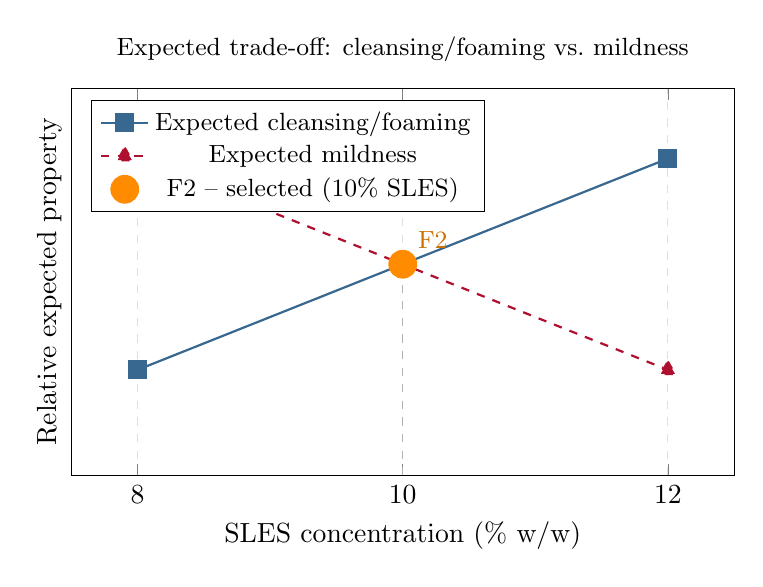
\begin{tikzpicture}
\begin{axis}[
  width=10cm, height=6.5cm,
  xlabel={SLES concentration (\% w/w)},
  ylabel={Relative expected property },
  xmin=7.5, xmax=12.5,
  ymin=0, ymax=11,
  xtick={8,10,12},
  ytick=\empty,
  legend pos=north west,
  legend style={font=\small},
  grid=both, grid style={dashed,gray!25},
  title={\small Expected trade-off: cleansing/foaming vs.\ mildness
         },
  title style={font=\small},
]
\addplot[thick, SteelBlue!80!black, mark=square*, mark size=3pt]
  coordinates {(8,3)(10,6)(12,9)};
\addlegendentry{Expected cleansing/foaming}

\addplot[thick, Crimson!80!black, dashed, mark=triangle*, mark size=3pt]
  coordinates {(8,9)(10,6)(12,3)};
\addlegendentry{Expected mildness}

\addplot[only marks, mark=*, mark size=5pt, DarkOrange]
  coordinates {(10,6)};
\addlegendentry{F2 -- selected (10\% SLES)}

\node[font=\small, DarkOrange!80!black, above right=2pt and 2pt]
  at (axis cs:10,6) {F2};

\draw[dashed, gray!60] (axis cs:10,0) -- (axis cs:10,6);
\end{axis}
\end{tikzpicture}
\caption{Hypothesised trade-off between expected cleansing/foaming and
expected mildness across the SLES range studied  \citep{ananthapadmanabhan2004,subramanyan2004}.
F2 (10\% SLES) was the intermediate level selected for detailed
observation.}
\label{fig:sles}
\end{figure*}

\subsection{Preliminary evaluation}

The selected batch F2 was assessed by simple descriptive methods
(Table~\ref{tab:evaluation}). Observations were not quantified. The
number of observers, the number of replicates, the observation period and
the storage conditions were not recorded, and only one batch of F2 was
evaluated. Spreadability and skin feel were judged informally and
subjectively by application to skin; no formal or blinded sensory panel
was used. pH was not determined because a pH meter was unavailable,
although pH is important because skin-surface pH influences barrier
function \citep{schmid2006}. Viscosity was not measured because a
viscometer was unavailable. No salicylic-acid assay, neem-marker assay,
microbiological test, preservative efficacy test, stability study or
controlled clinical study was performed.

\begin{table*}[!htbp]
\centering

\renewcommand{\arraystretch}{1.3}
\begin{tabularx}{\textwidth}{>{\bfseries}lX}
\toprule
Parameter & Procedure \\
\midrule
Appearance        & Visual inspection of gel structure, colour and
                    uniformity \\
Clarity           & Visual inspection against a suitable background for
                    cloudiness or turbidity \\
Odour             & Organoleptic assessment \\
Colour            & Visual inspection \\
Visible particles & Visual inspection for undissolved particles, foreign
                    matter or plant residue \\
Phase separation  & Visual inspection for separation of liquid or gel
                    phases \\
Uniformity        & Visual inspection for differences in colour, texture
                    and consistency \\
Homogeneity       & Visual inspection and handling for lumps or
                    aggregates \\
Spreadability     & Informal assessment of ease of spreading on skin \\
Skin feel         & Informal subjective assessment of ease of spreading,
                    smoothness, stickiness, greasiness, after-feel and
                    ease of rinsing \\
pH                & 5.5 - 7.0  \\
Viscosity         & 1500 - 2000 cP \\
Foam height       & 50 - 100 mm \\
\bottomrule
\end{tabularx}
\caption{Descriptive evaluation procedures applied to F2}
\label{tab:evaluation}
\end{table*}

\subsection{Formulation selection}

F2 was designated the selected formulation for preliminary
observation because it showed the most balanced visual and sensory
characteristics among the batches during the laboratory work. While
evaluation data were recorded for F1 and F3, F2 is not presented as a
statistically or experimentally validated optimum. A definitive
optimization would evaluate all batches against predefined quantitative
criteria with replicate measurements.

% ============================================================
\section{RESULTS AND DISCUSSION}
% ============================================================

The qualitative and available quantitative observations recorded during the laboratory work are
reported (Table~\ref{tab:results}).

\begin{table*}[!htbp]
\centering

\renewcommand{\arraystretch}{1.3}
\begin{tabularx}{\textwidth}{lXXX}
\toprule
\textbf{Parameter} & \textbf{F1} & \textbf{F2 (selected)} & \textbf{F3} \\
\midrule
Appearance
  & Pale-green transparent gel & Pale-green transparent gel & Pale-green transparent gel \\
Clarity
  & Clear & Clear & Clear \\
Odour
  & Lime-like & Lime-like & Lime-like \\
Colour
  & Pale green & Pale green & Pale green \\
Visible particles
  & None observed & None observed & None observed \\
Phase separation
  & No visible separation & No visible separation & No visible separation \\
Uniformity
  & Uniform & Uniform & Uniform \\
Homogeneity
  & Homogeneous & Homogeneous; no visible lumps & Homogeneous \\
Spreadability
  & Fair (qualitative) & Good (qualitative) & Good (qualitative) \\
Skin feel
  & Pleasant; less foaming & Pleasant; subjectively moisturising & Pleasant; slightly drying \\
pH
  & 5.5 - 7.0 & 5.5 - 7.0 & 5.5 - 7.0 \\
Viscosity
  & 1400 - 1800 cP
  & 1500 - 2000 cP
  & 1600 - 2200 cP \\
Foam height
  & 50 mm & 90 mm & 100 mm \\
\bottomrule
\end{tabularx}
\caption{Observations for the three batches}
\label{tab:results}
\end{table*}

F2 was a pale-green, transparent, uniform gel with a lime-like odour. No
visible particles or visible phase separation were seen during the
observation period, and the gel appeared homogeneous without visible
lumps. Spreadability was judged good and the skin feel pleasant and
subjectively moisturising. The terms ``good'' and ``pleasant'' are
subjective descriptors; they are not measured performance and do not
demonstrate moisturization efficacy.


% ============================================================
\subsection*{Comparison with a Marketed Product}
% ============================================================

Himalaya Purifying Neem Face Wash was used as a descriptive commercial
reference because it is a neem-containing face wash marketed for
pimple-prone skin \citep{himalaya2026}. According to the manufacturer's
product information it is a soap-free formulation containing neem and
turmeric, is described as a gentle gel, is stated to be free from
parabens, and is intended for use with a lather, rinsed off and patted
dry \citep{himalaya2026}. Product information can differ between markets
and versions.

A published clinical study of this commercial product was an open-label,
single-centre, single-arm, four-week study in 120 subjects with
mild-to-moderate acne or oily skin without existing acne; 79\% and 72\%
of subjects showed a reduction or no new appearance of inflammatory and
non-inflammatory lesions, respectively \citep{yogesh2022}. The study had
no comparator arm and was sponsored by the manufacturer, and its findings
relate only to that product. They cannot be used as evidence of efficacy
for the formulation developed here. Table~\ref{tab:comparison} presents a descriptive comparison between the developed formulation and the marketed reference.

\begin{table*}[!htbp]
\centering

\renewcommand{\arraystretch}{1.3}
\begin{tabularx}{\textwidth}{lXX}
\toprule
\textbf{Parameter} &
\textbf{Developed formulation (F2)} &
\textbf{Himalaya Purifying Neem Face Wash \citep{himalaya2026}} \\
\midrule
Dosage form
  & Transparent gel face wash & Gel face wash (per manufacturer) \\
Principal active concept
  & Salicylic acid + fresh aqueous neem extract & Neem + turmeric \\
Neem source
  & Freshly prepared aqueous extract 
  & Commercial ingredient \\
Preservative
  & Methyl paraben & Stated to be paraben-free \\
Intended skin
  & Oily / acne-prone skin
  & Pimple-prone skin (other skin types as stated) \\
pH
  & 5.5 - 7.0  & 6.9 \\
Viscosity
  & 1500 - 2000 cP & 1690 cP \\
Foam height
  & 90 mm & 98 mm \\

\bottomrule
\end{tabularx}
\caption{Descriptive comparison }
\label{tab:comparison}
\end{table*}

No comparative efficacy, safety, stability or microbiological conclusion
should be drawn from this comparison. The two products differ in
composition, preservative system, manufacturing controls and
characterization.


% ============================================================
\subsection*{Discussion}
\label{sec:discussion}
% ============================================================

This work shows that a laboratory-scale transparent gel face wash
containing salicylic acid and freshly prepared aqueous neem extract can
be prepared. The selected batch F2 was visually clear, pale green,
uniform and free of visible particles, with no visible phase separation
during the observation period. These observations describe the appearance
of the preparation and are consistent with, but do not prove, physical
compatibility of the ingredients. They cannot replace a formal stability
study.

The formulation concept is plausible from a formulation standpoint.
Salicylic acid has established desmolytic and comedolytic properties
\citep{decker2012,arif2015} and is conditionally recommended as a topical
option in current guidance \citep{reynolds2024}, while neem has been
investigated for several biological activities
\citep{singh2021,kumar2013,gupta2017,alzohairy2016}. However,
literature-supported mechanisms cannot substitute for testing the finished
formulation, and no activity of this rinse-off product was measured.

SLES concentration was the only planned variable. An intermediate level
was carried forward as it presented the best balance of characteristics.
The observed data suggest that lower SLES (F1) reduced foaming (50 mm),
and higher SLES (F3) increased foaming (100 mm) but felt slightly drying,
aligning with the expectation that higher SLES may reduce mildness
\citep{ananthapadmanabhan2004,subramanyan2004}. Selecting F2 for detailed
observation is a working decision, providing a balanced trade-off.

The absence of pH and viscosity data is a substantive limitation because
these properties are linked in this system. Carbomer gel rheology depends
on the degree and pH of neutralization \citep{islam2004}, and only about
1--2 drops of triethanolamine were used. In addition, salicylic acid is a
weak organic acid, so the pH reached after neutralizing the Carbopol will
influence how much of it is ionized and therefore its behaviour in
lipid-rich follicular material; this should be examined rather than
assumed. The final pH is also relevant to skin compatibility, since
skin-surface pH is acidic (below 5 on average) \citep{lambers2006},
influences barrier function \citep{schmid2006}, and has been reported to
be higher in acne \citep{prakash2017}. Calibrated pH measurement and
standardized viscosity or rheology determination are therefore priorities,
as is a clear identification of the lime water used (for example, calcium
hydroxide solution or a citrus preparation), because its nature would
affect pH and compatibility.

Fresh neem extract is a further source of variability. Plant material,
extraction conditions and phytochemical composition can vary, and herbal
dermatological products are prone to variability in ingredient
concentration and to quality-control and regulatory challenges
\citep{brar2025}. Because the extraction parameters and yield were not
recorded and no marker assay was done, the amount of any neem constituent
in the finished gel is unknown.

The preservation system needs particular attention. Methyl paraben is a
long-established preservative \citep{soni2002}, but the 1.5\% w/w used
here is nearly four times the 0.4\% (as acid) maximum permitted for a
single paraben ester in the European Union (Regulation~(EC)
No~1223/2009, Annex~V). The limits applicable in the intended market (for
example, under Indian requirements) should be checked, and the
preservative level or system should be revised before further development.
An aqueous botanical extract also raises the risk of microbial growth, so
microbiological quality and preservative efficacy must be tested before
any safety conclusion is made. Salicylic acid is itself a restricted
ingredient in some regulatory frameworks, with concentration and
product-type conditions, which should likewise be confirmed for the target
market.

The marketed-product comparison is descriptive only. The developed
formulation and the commercial product differ in active concept,
surfactant and preservative systems, manufacturing controls and
characterization, and clinical information on the commercial product
\citep{yogesh2022}, which comes from an uncontrolled study sponsored by
its manufacturer, cannot be transferred to the present formulation.

% 
Figure~\ref{fig:further} summarizes the work completed and the further
work needed to address these limitations.

%% ------ Figure 8 : Done vs. further work ------------------
\begin{figure*}[t]
\centering
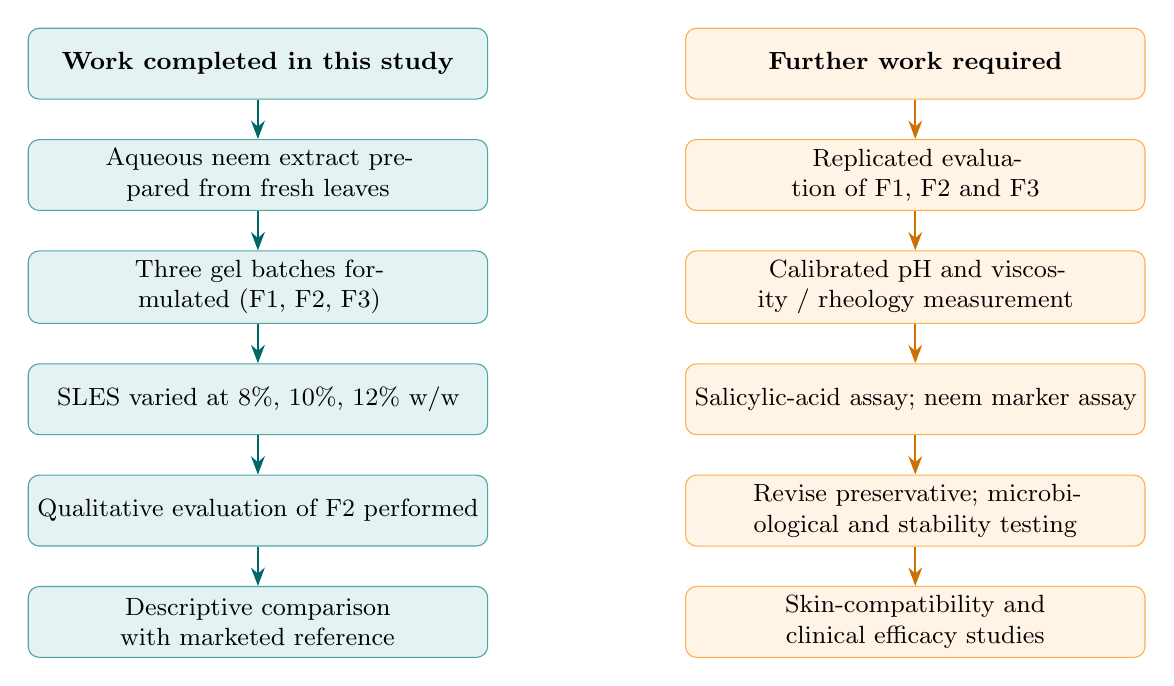
\begin{tikzpicture}[node distance=0.5cm]
  % Done column header
  \node[donebox, font=\small\bfseries] (dh)
    {Work completed in this study};
  \node[donebox, below=of dh] (d1)
    {Aqueous neem extract prepared from fresh leaves};
  \node[donebox, below=of d1] (d2)
    {Three gel batches formulated (F1, F2, F3)};
  \node[donebox, below=of d2] (d3)
    {SLES varied at 8\%, 10\%, 12\% w/w};
  \node[donebox, below=of d3] (d4)
    {Qualitative evaluation of F2 performed};
  \node[donebox, below=of d4] (d5)
    {Descriptive comparison with marketed reference};

  % Further work column header
  \node[todobox, right=2.5cm of dh, font=\small\bfseries] (th)
    {Further work required};
  \node[todobox, right=2.5cm of d1] (t1)
    {Replicated evaluation of F1, F2 and F3};
  \node[todobox, right=2.5cm of d2] (t2)
    {Calibrated pH and viscosity / rheology measurement};
  \node[todobox, right=2.5cm of d3] (t3)
    {Salicylic-acid assay; neem marker assay};
  \node[todobox, right=2.5cm of d4] (t4)
    {Revise preservative; microbiological and stability testing};
  \node[todobox, right=2.5cm of d5] (t5)
    {Skin-compatibility and clinical efficacy studies};

  \foreach \a/\b in {dh/d1,d1/d2,d2/d3,d3/d4,d4/d5}
    \draw[myarrow, Teal!80!black] (\a)--(\b);
  \foreach \a/\b in {th/t1,t1/t2,t2/t3,t3/t4,t4/t5}
    \draw[myarrow, DarkOrange!80!black] (\a)--(\b);
\end{tikzpicture}
\caption{Work completed in this study (left, teal) and further work
recommended to address its limitations (right, orange).}
\label{fig:further}
\end{figure*}

% ============================================================
\subsection*{Recommended Further Experimental Work}
% ============================================================

To move from preliminary laboratory feasibility towards a publishable
formulation-development study, the work in Table~\ref{tab:furtherwork}
is recommended.

\begin{table*}[!htbp]
\centering

\renewcommand{\arraystretch}{1.3}
\begin{tabularx}{\textwidth}{XX}
\toprule
\textbf{Study} & \textbf{Purpose} \\
\midrule
Replicated evaluation of F1, F2 and F3 against predefined criteria
  & Allow an evidence-based comparison of SLES concentrations \\
Calibrated pH measurement
  & Characterize acidity and reproducibility; relate pH to
    salicylic-acid ionization and skin compatibility \\
Instrumental viscosity / rheology
  & Quantify flow and gel characteristics \\
Quantitative salicylic-acid assay
  & Confirm active content and batch consistency \\
Neem marker / phytochemical characterization and recorded extraction
parameters
  & Improve botanical reproducibility \\
Revision of the preservative level or system, then microbiological
quality and preservative efficacy testing
  & Address regulatory limits and protection of an aqueous botanical
    formulation \\
Accelerated and long-term stability
  & Assess physical and chemical stability \\
Skin-compatibility testing under an ethics-approved protocol
  & Investigate tolerability \\
Validated anti-acne efficacy study
  & Determine whether the finished rinse-off product gives a measurable
    benefit \\
\bottomrule
\end{tabularx}
\caption{Recommended further studies}
\label{tab:furtherwork}
\end{table*}

% ============================================================
\section{CONCLUSION}
% ============================================================

A laboratory-scale transparent gel face wash containing salicylic acid
and freshly prepared neem extract was developed. Three batches were
designed with SLES at 8\%, 10\% and 12\% w/w, and the 10\% batch (F2)
was selected for preliminary detailed observation. F2 was visually
clear, pale green, uniform and free of visible particles, with no visible
phase separation and good qualitative spreadability.

The study supports the feasibility of preparing the formulation at
laboratory scale. It does not establish that F2 is an experimentally
validated optimum, nor does it establish anti-acne efficacy, antimicrobial
activity, preservative effectiveness, stability, active content or safety.
The methyl paraben level should be revised, and pH, viscosity, assay,
microbiological, stability and clinical studies are required before any
such claims are made.

% ============================================================
\section*{DECLARATIONS}
% ============================================================

\noindent\textbf{Ethics approval:} No clinical study, human-participant
study or animal study was conducted. Skin-feel and spreadability were
assessed informally and subjectively; [the authors should confirm the
number of assessors and whether their institution or the target journal
requires ethics review of such informal assessment].

\medskip
\noindent\textbf{Data availability:} The observations reported are those
recorded during the laboratory work; no other datasets were generated.


% ============================================================
\bibliography{references}
% ============================================================

\end{document}
